\chapter{关系模型}

\section{关系基本概念}

\begin{definition}[域(Domain)]
具有相同数据类型的一组值的集合.
如整数集合、字符串集合、全体学生集合.
\end{definition}

\begin{definition}[笛卡尔积(Cartesian Product)]
一组域$D_1,D_2,...,D_n$的\textcolor{red}{笛卡尔积}为:
\begin{align*}
    D_1\times D_2\times \cdots\times D_n = \{(d_1,d_2,...,d_n)|d_i\in D_i, i=1,2,...,n\}.
\end{align*}
笛卡尔积的元素$(d_1,d_2,...,d_n)$称作$n$元组(tuple).

元组的每一个值$d_i$被称作分量(component).

若$D_i$的基数为$m_i$, 则笛卡尔积的基数为$\prod_{i=1}^{n}m_i$.
\end{definition}

\begin{definition}[关系]
笛卡尔积$D_1\times D_2\times \cdots\times D_n$的子集称作在域$D_1,D_2,...,D_n$上的\textcolor{red}{关系}. 用$R(D_1,D_2,...,D_n)$表示. $R$是关系的名字, $n$是关系的度或目.

关系是笛卡尔积中\textcolor{red}{有意义}的子集.
\end{definition}

关系的性质:
\begin{enumerate}
    \item $P_1$: 列是同质的, 是同一类型的数据, 即每一列中的分量来自同一域.
    \item $P_2$: 不同的列可以来自同一域, 每列必须有不同的属性名. (一元联系、类型相同的属性)
    \item $P_3$: 行列的顺序无关紧要.
    \item $P_4$: 任意两个元组不能完全相同 (集合内不能有相同的两个元素)
    \item $P_5$: 每一分量必须是不可再分的数据, 称其为作满足第一范式(1NF)的关系. 
\end{enumerate}

\section{关系模型三要素}

关系模型的三要素:
\begin{enumerate}
    \item 数据结构.
    \item 数据操作.
    \item 数据完整性.
\end{enumerate}

\subsection{数据结构}

关系模型的数据结构就是\textcolor{red}{关系}: 实体集和联系都表示为关系.

\begin{definition}[候选码(Candidate Key)]
关系中的一个属性组, 其值能唯一标识一个元组. 
若从属性组去掉任何一个属性, 它就不具有这一性质了, 这样的属性组称为候选码.
\end{definition}

\begin{definition}[主属性]
任何一个候选码中的属性被称为主属性.
\end{definition}

\begin{definition}[主码(Priamry Key, PK)]
进行数据库设计时, 从一个关系的多个候选码中选定一个作为主码.
\end{definition}

\begin{definition}[外码(Foreign Key, FK)]
关系$R$中的一个属性组, 它不是$R$的码, 但它与另一个关系$S$的码相
对应, 称这个属性组为$R$的外码.
\end{definition}

\begin{definition}[关系模式]
关系的描述, 记为$R(A_1,A_2,...,A_n)$, 包括:
\begin{enumerate}
    \item 关系名、关系中的属性名.
    \item 属性向域的映像, 通常说明为属性的类型、长度等.
    \item 属性间的数据依赖关系, 比如在特定的时间和教室只能安排一门课.
\end{enumerate}
关系模式是稳定的.
\end{definition}

\begin{definition}[关系]
关系是某一时刻对应某个关系模式的内容(元组的集合). 关系是某一时刻的值, 是随时间不断变化的.
\end{definition}

\begin{definition}[关系型数据库]
\begin{enumerate}
    \item 型: 关系模式的集合, 数据库描述. 数据库的内涵(Intension).
    \item 值: 是某一时刻关系的集合. 数据库的外延(Extension).
\end{enumerate}
\end{definition}

\subsection{数据操作}

关系操作是集合操作. 操作的对象及结果都是集合. 是一次一集合 (Set-at-a-time)的方式.

非关系型的数据操作方式是一次一记录(Record-at-a-time).

关系数据语言的特点:
\begin{enumerate}
    \item 一体化: 对象单一, 都是关系, 因此操作符也单一
    \item 非过程化: 用户只需提出“做什么” , 无须说明“怎么做”. 存取路径的选择和操作过程由系统自动完成
    \item 面向集合的存取方式: 一次一关系.
\end{enumerate}

抽象的关系模型查询语言:
\begin{enumerate}
    \item 关系代数. 过程查询语言.
    \item 关系演算: 元组关系演算、域关系演算. 非过程查询语言.
\end{enumerate}

SQL(介于关系代数和关系验算之间, by IBM)、QUEL(基于 Codd 提出元组关系演算语言ALPHA)、QBE.

\subsection{数据完整性}

\begin{definition}[关系模型完整性]
关系模型完整性由三部分组成:
\begin{enumerate}
    \item 实体完整性
    \item 参照完整性
    \item 用户定义完整性
\end{enumerate}
\end{definition}

\begin{definition}[实体完整性]
关系的主码中的属性值不能为空值. (保证其实体存在.)
\end{definition}

\begin{definition}[参照完整性]
如果关系$R_2$的外码$F_k$与关系$R_1$的主码$P_k$相对应, 
则$R_2$中每个元组的$F_k$值或者等于$R_1$中某个元组的$P_k$值, 或者为空值.

如果关系$R_2$的某个元组$t_2$参照了关系$R_1$的某个元组$t_1$, 则$t_1$必须存在, 
也即必须与客观存在的实体发生联系.
\end{definition}

\begin{figure}[H]
    \centering
    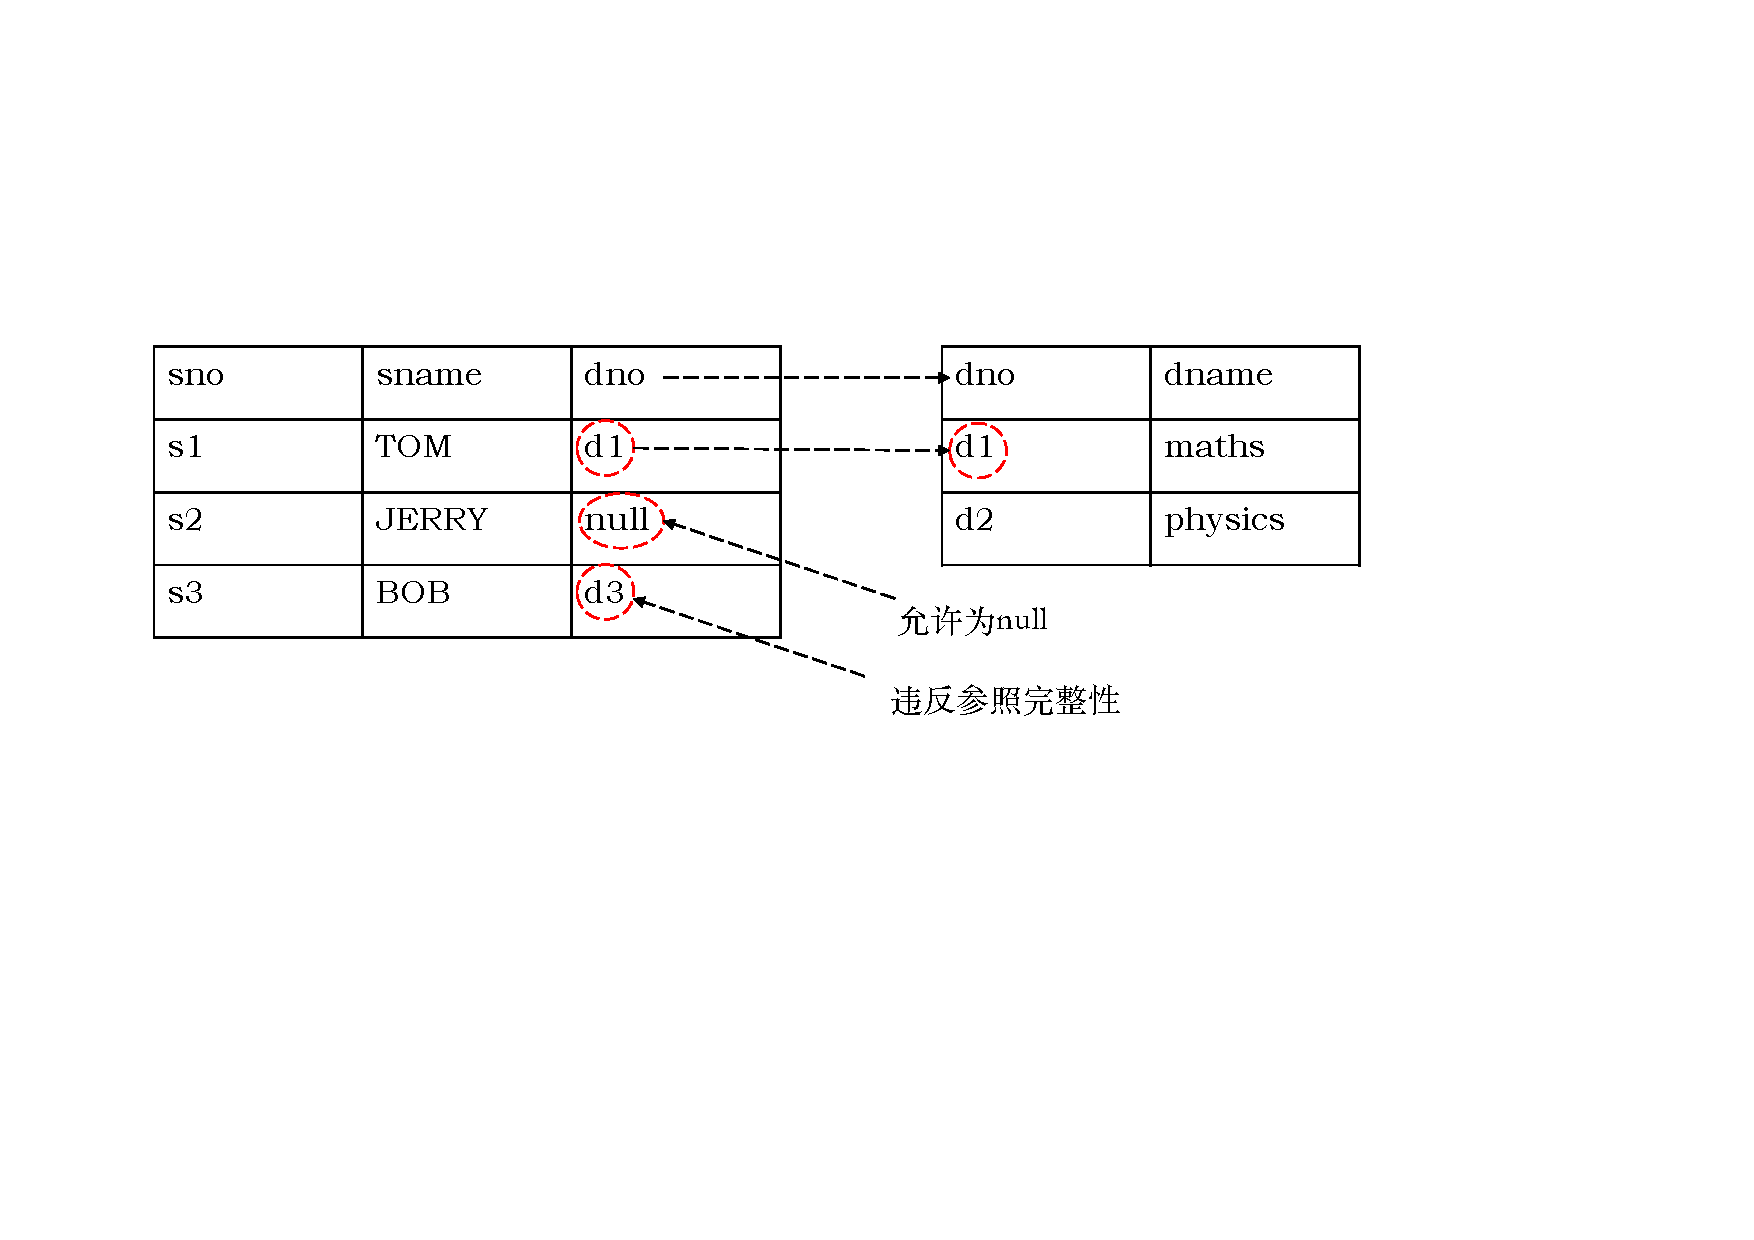
\includegraphics[width=.6\textwidth]{./figure/参照完整性.pdf}
    \caption{参照完整性}
\end{figure}

\begin{definition}[用户完整性]
用户针对具体应用环境定义的完整性约束条件.
\end{definition}

实体完整性和参照完整性由系统自动支持, 系统提供定义和检验用户定义的完整性的机制.

\section{关系代数运算}

\begin{figure}[H]
    \centering
    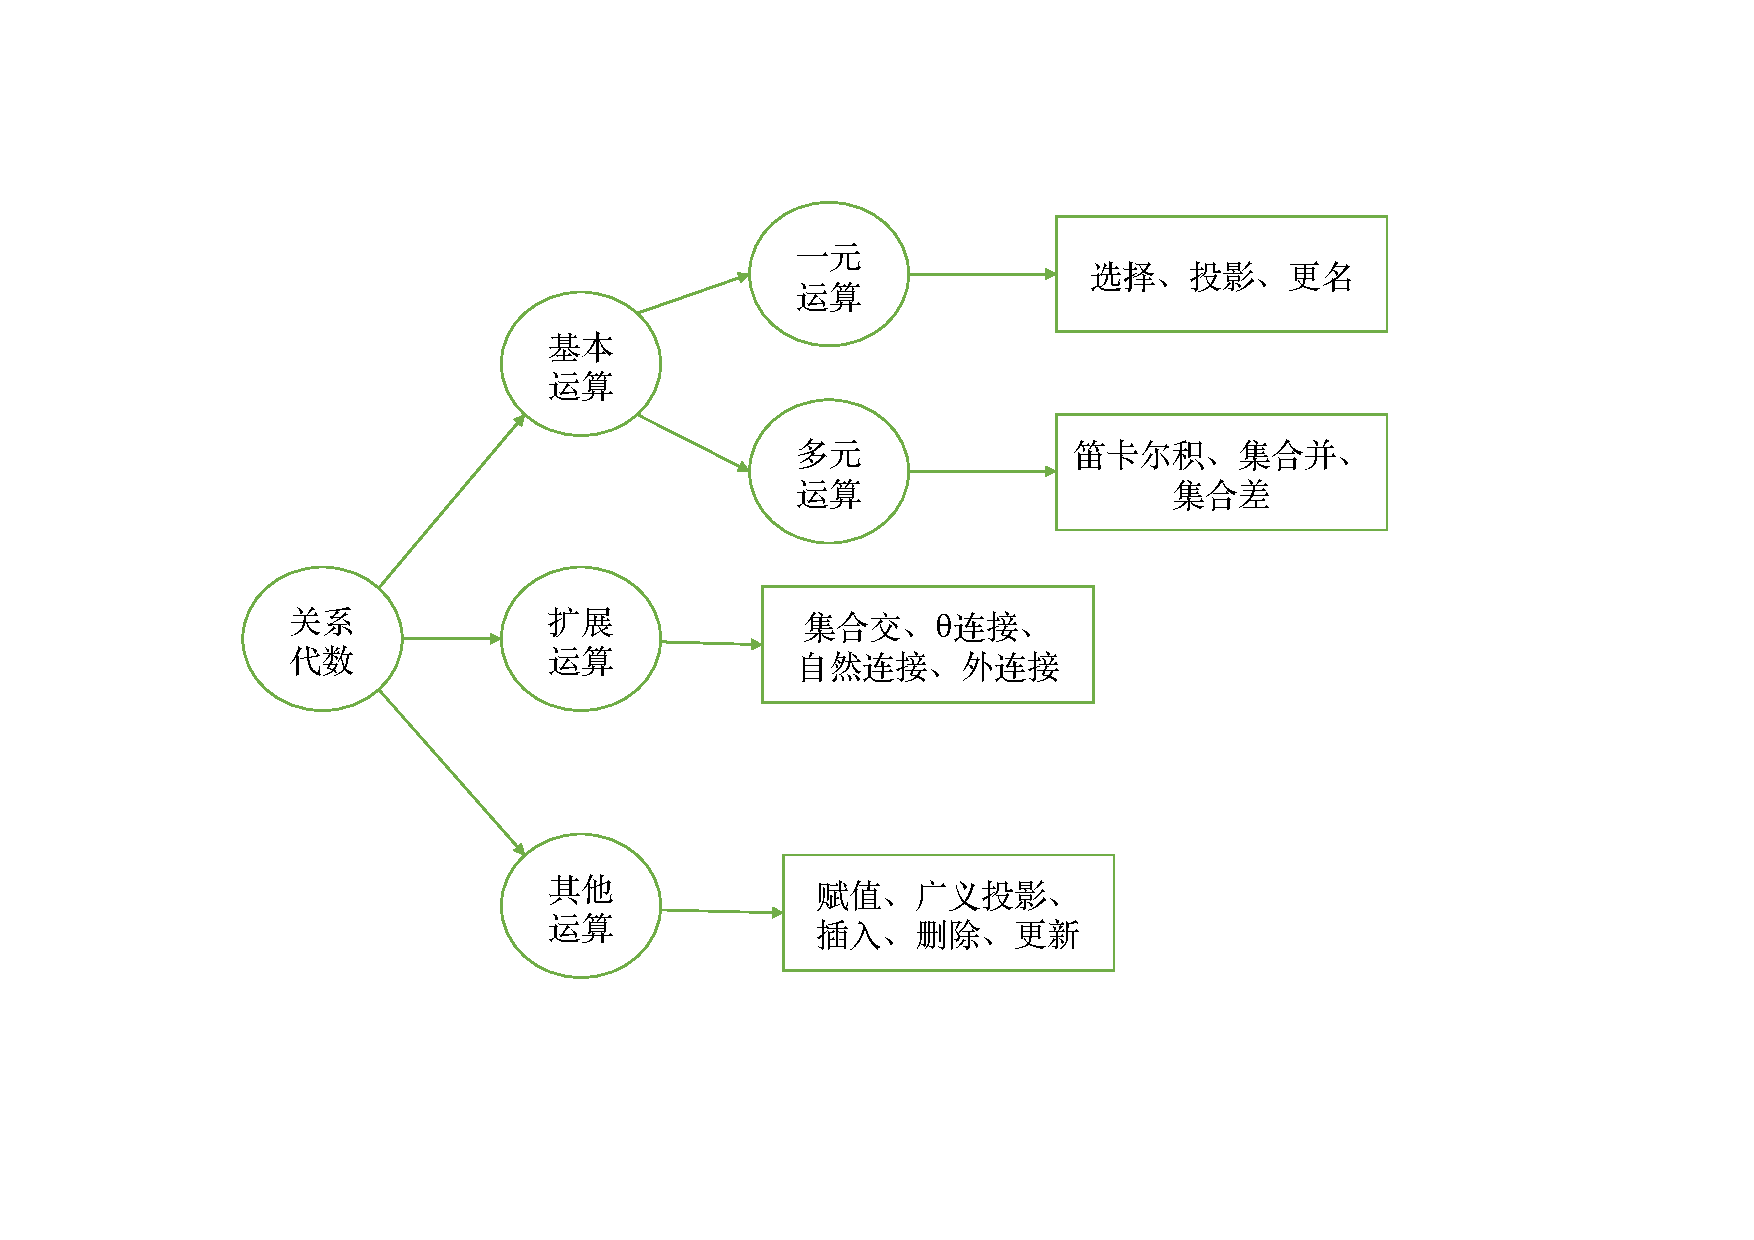
\includegraphics[width=.6\textwidth]{./figure/关系代数.pdf}
    \caption{关系代数示意图}
\end{figure}

\subsection{基本关系代数运算}

\subsubsection{一元运算}

\begin{definition}[选择运算]
在关系中选择给定条件的元组(行角度):
\begin{align*}
    \sigma_F(R)=\{t|t\in R,F(t)=\text{true}\}.
\end{align*}
$F$由逻辑运算符连接算术表达式而成.
\end{definition}

\begin{definition}[投影运算]
从关系中取若干列组成新的关系(从列的角度):
\begin{align*}
    \Pi_A(R) = \{t[A]|t\in R\}, A \subseteq R.
\end{align*}
\end{definition}

投影的结果要去掉相同的行:
\begin{figure}[H]
    \centering
    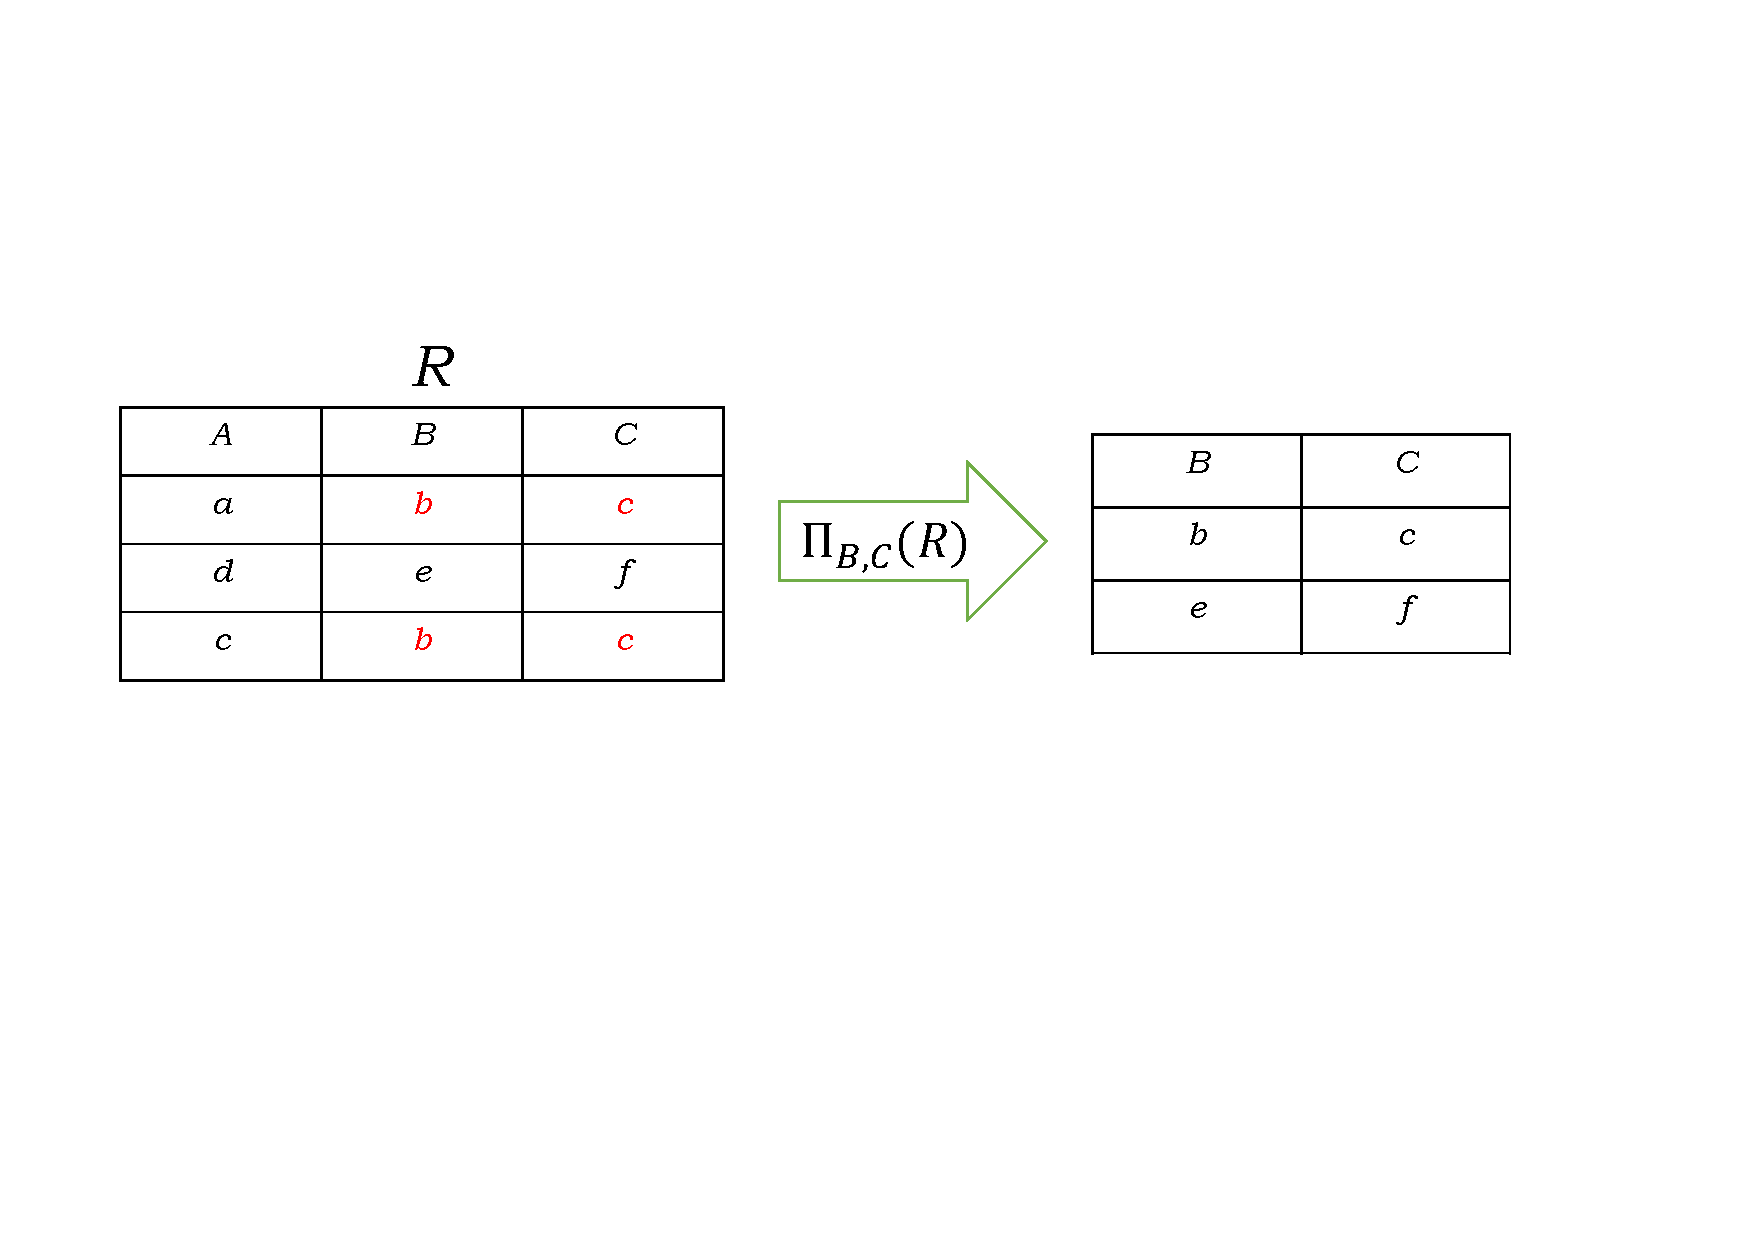
\includegraphics[width=.7\textwidth]{./figure/投影.pdf}
    \caption{投影运算要去掉相同的行}
\end{figure}

\begin{definition}[更名运算]
将关系$R$更名为$S: \rho_S(R)$; 将计算表达式$E$更名为关系$S: \rho_{S(A_1,A_2,...,A_n)}(E)$.
\begin{enumerate}
    \item 将更名运算施加到关系上, 得到具有不同名字的同一关系
    \item 当同一关系多次参与同一运算时需要更名
\end{enumerate}
\end{definition}


